\documentclass[twoside]{book}

% Packages required by doxygen
\usepackage{fixltx2e}
\usepackage{calc}
\usepackage{doxygen}
\usepackage[export]{adjustbox} % also loads graphicx
\usepackage{graphicx}
\usepackage[utf8]{inputenc}
\usepackage{makeidx}
\usepackage{multicol}
\usepackage{multirow}
\PassOptionsToPackage{warn}{textcomp}
\usepackage{textcomp}
\usepackage[nointegrals]{wasysym}
\usepackage[table]{xcolor}

% Font selection
\usepackage[T1]{fontenc}
\usepackage[scaled=.90]{helvet}
\usepackage{courier}
\usepackage{amssymb}
\usepackage{sectsty}
\renewcommand{\familydefault}{\sfdefault}
\allsectionsfont{%
  \fontseries{bc}\selectfont%
  \color{darkgray}%
}
\renewcommand{\DoxyLabelFont}{%
  \fontseries{bc}\selectfont%
  \color{darkgray}%
}
\newcommand{\+}{\discretionary{\mbox{\scriptsize$\hookleftarrow$}}{}{}}

% Page & text layout
\usepackage{geometry}
\geometry{%
  a4paper,%
  top=2.5cm,%
  bottom=2.5cm,%
  left=2.5cm,%
  right=2.5cm%
}
\tolerance=750
\hfuzz=15pt
\hbadness=750
\setlength{\emergencystretch}{15pt}
\setlength{\parindent}{0cm}
\setlength{\parskip}{3ex plus 2ex minus 2ex}
\makeatletter
\renewcommand{\paragraph}{%
  \@startsection{paragraph}{4}{0ex}{-1.0ex}{1.0ex}{%
    \normalfont\normalsize\bfseries\SS@parafont%
  }%
}
\renewcommand{\subparagraph}{%
  \@startsection{subparagraph}{5}{0ex}{-1.0ex}{1.0ex}{%
    \normalfont\normalsize\bfseries\SS@subparafont%
  }%
}
\makeatother

% Headers & footers
\usepackage{fancyhdr}
\pagestyle{fancyplain}
\fancyhead[LE]{\fancyplain{}{\bfseries\thepage}}
\fancyhead[CE]{\fancyplain{}{}}
\fancyhead[RE]{\fancyplain{}{\bfseries\leftmark}}
\fancyhead[LO]{\fancyplain{}{\bfseries\rightmark}}
\fancyhead[CO]{\fancyplain{}{}}
\fancyhead[RO]{\fancyplain{}{\bfseries\thepage}}
\fancyfoot[LE]{\fancyplain{}{}}
\fancyfoot[CE]{\fancyplain{}{}}
\fancyfoot[RE]{\fancyplain{}{\bfseries\scriptsize Generated by Doxygen }}
\fancyfoot[LO]{\fancyplain{}{\bfseries\scriptsize Generated by Doxygen }}
\fancyfoot[CO]{\fancyplain{}{}}
\fancyfoot[RO]{\fancyplain{}{}}
\renewcommand{\footrulewidth}{0.4pt}
\renewcommand{\chaptermark}[1]{%
  \markboth{#1}{}%
}
\renewcommand{\sectionmark}[1]{%
  \markright{\thesection\ #1}%
}

% Indices & bibliography
\usepackage{natbib}
\usepackage[titles]{tocloft}
\setcounter{tocdepth}{3}
\setcounter{secnumdepth}{5}
\makeindex

% Hyperlinks (required, but should be loaded last)
\usepackage{ifpdf}
\ifpdf
  \usepackage[pdftex,pagebackref=true]{hyperref}
\else
  \usepackage[ps2pdf,pagebackref=true]{hyperref}
\fi
\hypersetup{%
  colorlinks=true,%
  linkcolor=blue,%
  citecolor=blue,%
  unicode%
}

% Custom commands
\newcommand{\clearemptydoublepage}{%
  \newpage{\pagestyle{empty}\cleardoublepage}%
}

\usepackage{caption}
\captionsetup{labelsep=space,justification=centering,font={bf},singlelinecheck=off,skip=4pt,position=top}

%===== C O N T E N T S =====

\begin{document}

% Titlepage & ToC
\hypersetup{pageanchor=false,
             bookmarksnumbered=true,
             pdfencoding=unicode
            }
\pagenumbering{alph}
\begin{titlepage}
\vspace*{7cm}
\begin{center}%
{\Large Práctica \#06\+: Simulación de autómatas finitos deterministas }\\
\vspace*{1cm}
{\large Generated by Doxygen 1.8.13}\\
\end{center}
\end{titlepage}
\clearemptydoublepage
\pagenumbering{roman}
\tableofcontents
\clearemptydoublepage
\pagenumbering{arabic}
\hypersetup{pageanchor=true}

%--- Begin generated contents ---
\chapter{Práctica \#06\+: Simulación de autómatas finitos deterministas}
\label{md__r_e_a_d_m_e}
\Hypertarget{md__r_e_a_d_m_e}
\subsection*{Objetivo}

Esta práctica consistirá en la realización de un programa escrito en C++ que lea desde un fichero las especificaciones de un autómata finito determinista (D\+FA) y, a continuación, simule el comportamiento del autómata para una cadena que se dé como entrada.

Fichero para la definición del autómata finito determinista El autómata finito determinista vendrá definido en un fichero de texto con extensión .dfa y que tendrá el siguiente formato\+:


\begin{DoxyItemize}
\item Línea 1\+: Número total de estados del D\+FA
\item Línea 2\+: Estado de arranque del D\+FA
\item A continuación vendrá una línea para cada uno de los estados. Cada línea contendrá los siguientes números, separados entre sí por espacios en blanco\+:
\begin{DoxyItemize}
\item Número identificador del estado. Los estados del autómata se representarán mediante números enteros sin signo. La numeración de los estados corresponderá a los primeros números naturales comenzando por 0.
\item Un 1 si se trata de un estado de aceptación y un 0 si se trata de un estado de no aceptación.
\item Número de transiciones que posee el estado.
\item A continuación, para cada una de las transiciones, y separados por espacios en blanco, se detallará la información siguiente\+:
\begin{DoxyItemize}
\item Símbolo de entrada necesario para que se produzca la transición.
\item Estado destino de la transición.
\end{DoxyItemize}
\end{DoxyItemize}
\end{DoxyItemize}

A modo de ejemplo, se muestra un autómata junto con la definición del mismo especificada mediante un fichero .dfa



El programa deberá detectar que no haya ningún error en la definición del autómata. Esto es, habría que analizar que se cumplen las siguientes condiciones\+:


\begin{DoxyItemize}
\item Existe uno y sólo un estado inicial para el autómata.
\item Para cada estado del autómata siempre existe una y sólo una transición para cada uno de los símbolos del alfabeto.
\end{DoxyItemize}

\subsection*{Funcionamiento general del programa}

El programa principal debería ofrecer al usuario las siguientes opciones\+:


\begin{DoxyItemize}
\item Leer D\+FA\+: al seleccionar esta opción se deberá solicitar al usuario que introduzca el nombre del fichero .dfa donde se encuentra la especificación del autómata. A continuación, se deberá crear el autómata a partir de la especificación dada en el fichero. Habrá que notificar al usuario si se produce algún error en la creación del D\+FA.
\item Mostrar D\+FA\+: al seleccionar esta opción se mostrará por pantalla el D\+FA actualmente definido (previamente leído de fichero) en nuestro programa. Para mostrar el D\+FA por pantalla se seguirá el formato establecido para los ficheros .dfa
\item Identificar estados de muerte\+: al seleccionar esta opción se deberá mostrar por pantalla si el autómata previamente definido tiene estados de muerte y si es así, habrá que indicar cuáles son los identificadores de dichos estados de muerte.
\item Analizar cadena\+: al seleccionar esta opción se deberá solicitar al usuario que introduzca una cadena. Para la cadena indicada por el usuario se deberá determinar si es aceptada o no por el autómata actualmente definido. Al igual que ocurre con las dos opciones anteriores, esta opción tampoco se podrá ejecutar hasta que se haya definido un D\+FA. El formato de la traza a mostrar por pantalla será el siguiente\+: \begin{DoxyVerb}      Cadena de entrada: ___________
      Estado actual    Entrada    Siguiente estado
      X                Y          Z
      X                Y          Z
      X                Y          Z
      Cadena de entrada ACEPTADA / NO ACEPTADA
\end{DoxyVerb}

\end{DoxyItemize}

Tal y como se indica en las líneas anteriores, en primer lugar se deberá mostrar la cadena de entrada. A continuación se indicará cómo va transitando de un estado a otro el autómata según va leyendo la cadena de entrada y finalmente, se deberá mostrar el mensaje “\+Cadena de entrada A\+C\+E\+P\+T\+A\+D\+A” si la cadena de entrada es aceptada por el D\+FA o el mensaje “\+Cadena de entrada NO A\+C\+E\+P\+T\+A\+D\+A” si la cadena de entrada no es aceptada por el D\+FA.

\subsection*{Detalles de implementación}


\begin{DoxyItemize}
\item Para la implementación de esta práctica se deberá definir una clase D\+FA que proporcione al menos los métodos necesarios para leer e inicializar un D\+FA desde un fichero, para mostrar un D\+FA, para identificar los estados de muerte del D\+FA y para realizar una traza de las transiciones llevadas a cabo cuando se da como entrada una determinada cadena.
\item También se deberá definir una clase \char`\"{}\+Estado\char`\"{} que agrupe las características correspondientes al estado de un D\+FA y las funcionalidades asociadas. Se valorará un buen diseño orientado a objetos basado en la definición formal de un D\+FA (\char`\"{}... un automata finito determinista D\+F\+A se define como un conjunto de estados ....\char`\"{} )
\item Se requerirá el uso de Makefiles para compilar los códigos.
\item Se requerirán los códigos de cada clase en archivos separados (cada clase con su .h y su .cpp) 
\end{DoxyItemize}
\chapter{Class Index}
\section{Class List}
Here are the classes, structs, unions and interfaces with brief descriptions\+:\begin{DoxyCompactList}
\item\contentsline{section}{\hyperlink{class_dfa}{Dfa} }{\pageref{class_dfa}}{}
\item\contentsline{section}{\hyperlink{class_state}{State} }{\pageref{class_state}}{}
\item\contentsline{section}{\hyperlink{class_transition}{Transition} }{\pageref{class_transition}}{}
\end{DoxyCompactList}

\chapter{File Index}
\section{File List}
Here is a list of all files with brief descriptions\+:\begin{DoxyCompactList}
\item\contentsline{section}{include/\hyperlink{_dfa_8hpp}{Dfa.\+hpp} }{\pageref{_dfa_8hpp}}{}
\item\contentsline{section}{include/\hyperlink{_state_8hpp}{State.\+hpp} }{\pageref{_state_8hpp}}{}
\item\contentsline{section}{include/\hyperlink{_transition_8hpp}{Transition.\+hpp} }{\pageref{_transition_8hpp}}{}
\item\contentsline{section}{src/\hyperlink{_dfa_8cpp}{Dfa.\+cpp} }{\pageref{_dfa_8cpp}}{}
\item\contentsline{section}{src/\hyperlink{_main_8cpp}{Main.\+cpp} }{\pageref{_main_8cpp}}{}
\item\contentsline{section}{src/\hyperlink{_state_8cpp}{State.\+cpp} }{\pageref{_state_8cpp}}{}
\item\contentsline{section}{src/\hyperlink{_transition_8cpp}{Transition.\+cpp} }{\pageref{_transition_8cpp}}{}
\end{DoxyCompactList}

\chapter{Class Documentation}
\hypertarget{class_dfa}{}\section{Dfa Class Reference}
\label{class_dfa}\index{Dfa@{Dfa}}


{\ttfamily \#include $<$Dfa.\+hpp$>$}

\subsection*{Public Member Functions}
\begin{DoxyCompactItemize}
\item 
\hyperlink{class_dfa_a8b4306c41ff0004264f56563e4399992}{Dfa} ()
\begin{DoxyCompactList}\small\item\em Construct a new \hyperlink{class_dfa}{Dfa}\+:\+: \hyperlink{class_dfa}{Dfa} object Constructor por defecto. \end{DoxyCompactList}\item 
\hyperlink{class_dfa_a2d110a2cc46b2dab6e6f9e901639b0cd}{$\sim$\+Dfa} ()
\begin{DoxyCompactList}\small\item\em Destroy the \hyperlink{class_dfa}{Dfa}\+:\+: \hyperlink{class_dfa}{Dfa} object Destructor. \end{DoxyCompactList}\item 
void \hyperlink{class_dfa_ae04b47677350573031c492799a1c897b}{clear} ()
\begin{DoxyCompactList}\small\item\em Limpiar D\+FA. \end{DoxyCompactList}\item 
bool \hyperlink{class_dfa_a54b373da1b88485641d0aa0e5fa303dd}{read\+\_\+dfa} (const string \&)
\begin{DoxyCompactList}\small\item\em Leer D\+FA del fichero. \end{DoxyCompactList}\item 
const set$<$ \hyperlink{class_state}{State} $>$ \& \hyperlink{class_dfa_a5f6b650f05ec3b8a5aa862c0f513c19e}{getallstates} ()
\begin{DoxyCompactList}\small\item\em Obtener el conjunto de estados. \end{DoxyCompactList}\item 
const set$<$ \hyperlink{class_state}{State} $>$ \hyperlink{class_dfa_a5e6cfb28034248d381e2fedb0df3d377}{get\+\_\+death\+\_\+states} () const
\begin{DoxyCompactList}\small\item\em Obtener conjunto de estados de muerte. \end{DoxyCompactList}\item 
bool \hyperlink{class_dfa_a0dd99d06e33e16c8fd342af4dbba3551}{check\+\_\+string} (const string \&)
\begin{DoxyCompactList}\small\item\em Comprobar si el D\+FA genera la cadena. \end{DoxyCompactList}\item 
const set$<$ char $>$ \hyperlink{class_dfa_a4483dc3db82de29855237b13a63c42cd}{get\+\_\+alphabet} () const
\begin{DoxyCompactList}\small\item\em Getter del alfabeto del D\+FA. \end{DoxyCompactList}\end{DoxyCompactItemize}
\subsection*{Friends}
\begin{DoxyCompactItemize}
\item 
ostream \& \hyperlink{class_dfa_ae4bcdc6c0f5c2374f14902fd5e073c7d}{operator$<$$<$} (ostream \&os, const \hyperlink{class_dfa}{Dfa} \&dfa)
\end{DoxyCompactItemize}


\subsection{Detailed Description}


Definition at line 11 of file Dfa.\+hpp.



\subsection{Constructor \& Destructor Documentation}
\mbox{\Hypertarget{class_dfa_a8b4306c41ff0004264f56563e4399992}\label{class_dfa_a8b4306c41ff0004264f56563e4399992}} 
\index{Dfa@{Dfa}!Dfa@{Dfa}}
\index{Dfa@{Dfa}!Dfa@{Dfa}}
\subsubsection{\texorpdfstring{Dfa()}{Dfa()}}
{\footnotesize\ttfamily Dfa\+::\+Dfa (\begin{DoxyParamCaption}{ }\end{DoxyParamCaption})}



Construct a new \hyperlink{class_dfa}{Dfa}\+:\+: \hyperlink{class_dfa}{Dfa} object Constructor por defecto. 



Definition at line 9 of file Dfa.\+cpp.

\mbox{\Hypertarget{class_dfa_a2d110a2cc46b2dab6e6f9e901639b0cd}\label{class_dfa_a2d110a2cc46b2dab6e6f9e901639b0cd}} 
\index{Dfa@{Dfa}!````~Dfa@{$\sim$\+Dfa}}
\index{````~Dfa@{$\sim$\+Dfa}!Dfa@{Dfa}}
\subsubsection{\texorpdfstring{$\sim$\+Dfa()}{~Dfa()}}
{\footnotesize\ttfamily Dfa\+::$\sim$\+Dfa (\begin{DoxyParamCaption}{ }\end{DoxyParamCaption})}



Destroy the \hyperlink{class_dfa}{Dfa}\+:\+: \hyperlink{class_dfa}{Dfa} object Destructor. 



Definition at line 16 of file Dfa.\+cpp.



\subsection{Member Function Documentation}
\mbox{\Hypertarget{class_dfa_a0dd99d06e33e16c8fd342af4dbba3551}\label{class_dfa_a0dd99d06e33e16c8fd342af4dbba3551}} 
\index{Dfa@{Dfa}!check\+\_\+string@{check\+\_\+string}}
\index{check\+\_\+string@{check\+\_\+string}!Dfa@{Dfa}}
\subsubsection{\texorpdfstring{check\+\_\+string()}{check\_string()}}
{\footnotesize\ttfamily bool Dfa\+::check\+\_\+string (\begin{DoxyParamCaption}\item[{const string \&}]{str }\end{DoxyParamCaption})}



Comprobar si el D\+FA genera la cadena. 


\begin{DoxyParams}{Parameters}
{\em str} & cadena \\
\hline
\end{DoxyParams}
\begin{DoxyReturn}{Returns}
true 

false 
\end{DoxyReturn}


Definition at line 175 of file Dfa.\+cpp.

Here is the call graph for this function\+:
\nopagebreak
\begin{figure}[H]
\begin{center}
\leavevmode
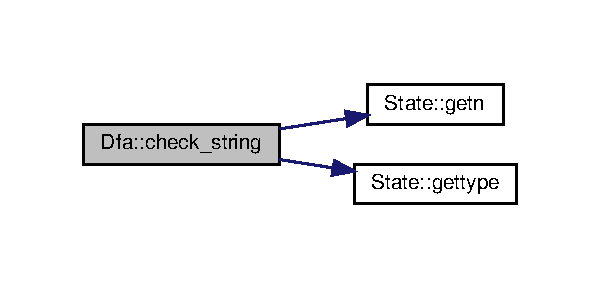
\includegraphics[width=288pt]{class_dfa_a0dd99d06e33e16c8fd342af4dbba3551_cgraph}
\end{center}
\end{figure}
Here is the caller graph for this function\+:
\nopagebreak
\begin{figure}[H]
\begin{center}
\leavevmode
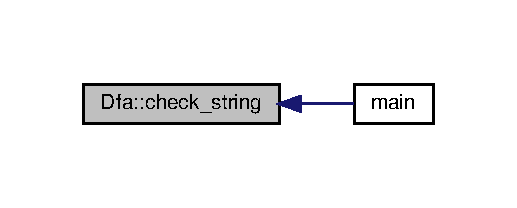
\includegraphics[width=248pt]{class_dfa_a0dd99d06e33e16c8fd342af4dbba3551_icgraph}
\end{center}
\end{figure}
\mbox{\Hypertarget{class_dfa_ae04b47677350573031c492799a1c897b}\label{class_dfa_ae04b47677350573031c492799a1c897b}} 
\index{Dfa@{Dfa}!clear@{clear}}
\index{clear@{clear}!Dfa@{Dfa}}
\subsubsection{\texorpdfstring{clear()}{clear()}}
{\footnotesize\ttfamily void Dfa\+::clear (\begin{DoxyParamCaption}{ }\end{DoxyParamCaption})}



Limpiar D\+FA. 



Definition at line 24 of file Dfa.\+cpp.

Here is the caller graph for this function\+:
\nopagebreak
\begin{figure}[H]
\begin{center}
\leavevmode
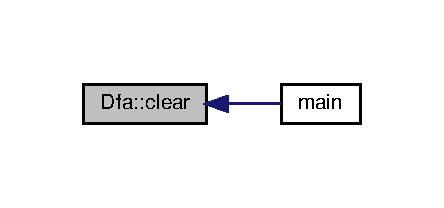
\includegraphics[width=213pt]{class_dfa_ae04b47677350573031c492799a1c897b_icgraph}
\end{center}
\end{figure}
\mbox{\Hypertarget{class_dfa_a4483dc3db82de29855237b13a63c42cd}\label{class_dfa_a4483dc3db82de29855237b13a63c42cd}} 
\index{Dfa@{Dfa}!get\+\_\+alphabet@{get\+\_\+alphabet}}
\index{get\+\_\+alphabet@{get\+\_\+alphabet}!Dfa@{Dfa}}
\subsubsection{\texorpdfstring{get\+\_\+alphabet()}{get\_alphabet()}}
{\footnotesize\ttfamily const set$<$ char $>$ Dfa\+::get\+\_\+alphabet (\begin{DoxyParamCaption}{ }\end{DoxyParamCaption}) const}



Getter del alfabeto del D\+FA. 

\begin{DoxyReturn}{Returns}
const set$<$char$>$ 
\end{DoxyReturn}


Definition at line 164 of file Dfa.\+cpp.

Here is the caller graph for this function\+:
\nopagebreak
\begin{figure}[H]
\begin{center}
\leavevmode
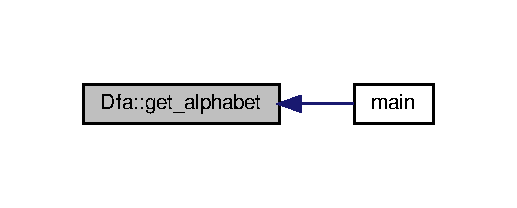
\includegraphics[width=248pt]{class_dfa_a4483dc3db82de29855237b13a63c42cd_icgraph}
\end{center}
\end{figure}
\mbox{\Hypertarget{class_dfa_a5e6cfb28034248d381e2fedb0df3d377}\label{class_dfa_a5e6cfb28034248d381e2fedb0df3d377}} 
\index{Dfa@{Dfa}!get\+\_\+death\+\_\+states@{get\+\_\+death\+\_\+states}}
\index{get\+\_\+death\+\_\+states@{get\+\_\+death\+\_\+states}!Dfa@{Dfa}}
\subsubsection{\texorpdfstring{get\+\_\+death\+\_\+states()}{get\_death\_states()}}
{\footnotesize\ttfamily const set$<$ \hyperlink{class_state}{State} $>$ Dfa\+::get\+\_\+death\+\_\+states (\begin{DoxyParamCaption}{ }\end{DoxyParamCaption}) const}



Obtener conjunto de estados de muerte. 

\begin{DoxyReturn}{Returns}
const set$<$\+State$>$ 
\end{DoxyReturn}


Definition at line 144 of file Dfa.\+cpp.

Here is the caller graph for this function\+:
\nopagebreak
\begin{figure}[H]
\begin{center}
\leavevmode
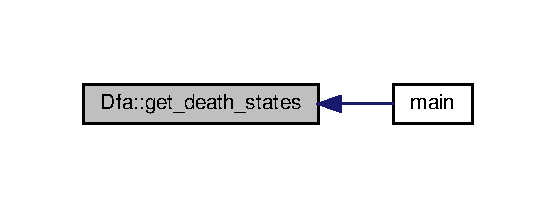
\includegraphics[width=267pt]{class_dfa_a5e6cfb28034248d381e2fedb0df3d377_icgraph}
\end{center}
\end{figure}
\mbox{\Hypertarget{class_dfa_a5f6b650f05ec3b8a5aa862c0f513c19e}\label{class_dfa_a5f6b650f05ec3b8a5aa862c0f513c19e}} 
\index{Dfa@{Dfa}!getallstates@{getallstates}}
\index{getallstates@{getallstates}!Dfa@{Dfa}}
\subsubsection{\texorpdfstring{getallstates()}{getallstates()}}
{\footnotesize\ttfamily const set$<$ \hyperlink{class_state}{State} $>$ \& Dfa\+::getallstates (\begin{DoxyParamCaption}{ }\end{DoxyParamCaption})}



Obtener el conjunto de estados. 

\begin{DoxyReturn}{Returns}
const set$<$\+State$>$\& 
\end{DoxyReturn}


Definition at line 135 of file Dfa.\+cpp.

\mbox{\Hypertarget{class_dfa_a54b373da1b88485641d0aa0e5fa303dd}\label{class_dfa_a54b373da1b88485641d0aa0e5fa303dd}} 
\index{Dfa@{Dfa}!read\+\_\+dfa@{read\+\_\+dfa}}
\index{read\+\_\+dfa@{read\+\_\+dfa}!Dfa@{Dfa}}
\subsubsection{\texorpdfstring{read\+\_\+dfa()}{read\_dfa()}}
{\footnotesize\ttfamily bool Dfa\+::read\+\_\+dfa (\begin{DoxyParamCaption}\item[{const string \&}]{path }\end{DoxyParamCaption})}



Leer D\+FA del fichero. 


\begin{DoxyParams}{Parameters}
{\em path} & ruta del fichero \\
\hline
\end{DoxyParams}
\begin{DoxyReturn}{Returns}
true 

false 
\end{DoxyReturn}


Definition at line 40 of file Dfa.\+cpp.

Here is the call graph for this function\+:
\nopagebreak
\begin{figure}[H]
\begin{center}
\leavevmode
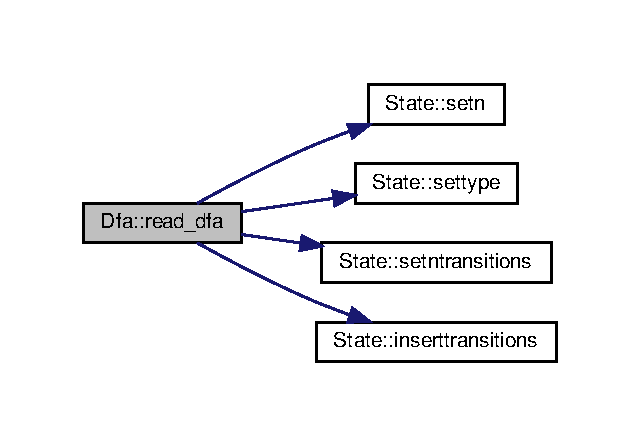
\includegraphics[width=307pt]{class_dfa_a54b373da1b88485641d0aa0e5fa303dd_cgraph}
\end{center}
\end{figure}
Here is the caller graph for this function\+:
\nopagebreak
\begin{figure}[H]
\begin{center}
\leavevmode
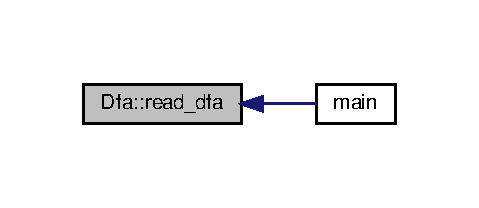
\includegraphics[width=230pt]{class_dfa_a54b373da1b88485641d0aa0e5fa303dd_icgraph}
\end{center}
\end{figure}


\subsection{Friends And Related Function Documentation}
\mbox{\Hypertarget{class_dfa_ae4bcdc6c0f5c2374f14902fd5e073c7d}\label{class_dfa_ae4bcdc6c0f5c2374f14902fd5e073c7d}} 
\index{Dfa@{Dfa}!operator$<$$<$@{operator$<$$<$}}
\index{operator$<$$<$@{operator$<$$<$}!Dfa@{Dfa}}
\subsubsection{\texorpdfstring{operator$<$$<$}{operator<<}}
{\footnotesize\ttfamily ostream\& operator$<$$<$ (\begin{DoxyParamCaption}\item[{ostream \&}]{os,  }\item[{const \hyperlink{class_dfa}{Dfa} \&}]{dfa }\end{DoxyParamCaption})\hspace{0.3cm}{\ttfamily [friend]}}



Definition at line 234 of file Dfa.\+cpp.



The documentation for this class was generated from the following files\+:\begin{DoxyCompactItemize}
\item 
include/\hyperlink{_dfa_8hpp}{Dfa.\+hpp}\item 
src/\hyperlink{_dfa_8cpp}{Dfa.\+cpp}\end{DoxyCompactItemize}

\hypertarget{class_state}{}\section{State Class Reference}
\label{class_state}\index{State@{State}}


{\ttfamily \#include $<$State.\+hpp$>$}

\subsection*{Public Member Functions}
\begin{DoxyCompactItemize}
\item 
\hyperlink{class_state_ab91bb1dd5aa6260ab2a456581daf9ec2}{State} ()
\begin{DoxyCompactList}\small\item\em Construct a new \hyperlink{class_state}{State}\+:\+: \hyperlink{class_state}{State} object Constructor por defecto. \end{DoxyCompactList}\item 
\hyperlink{class_state_a5ca97340266d486dfa42225f19c40de3}{State} (const \hyperlink{class_state}{State} \&)
\begin{DoxyCompactList}\small\item\em Construct a new \hyperlink{class_state}{State}\+:\+: \hyperlink{class_state}{State} object Constructor de copia. \end{DoxyCompactList}\item 
\hyperlink{class_state_afab438d92b90dc18d194dbd9c9c8bab3}{$\sim$\+State} ()
\begin{DoxyCompactList}\small\item\em Destroy the \hyperlink{class_state}{State}\+:\+: \hyperlink{class_state}{State} object Destructor. \end{DoxyCompactList}\item 
const unsigned int \& \hyperlink{class_state_ac045d201c81b6ea1ff3da734c6e286a7}{getn} ()
\begin{DoxyCompactList}\small\item\em Obtener el identificador del estado. \end{DoxyCompactList}\item 
const unsigned int \& \hyperlink{class_state_ad701488d3ba934847dcea6222d65719e}{gettype} ()
\begin{DoxyCompactList}\small\item\em Obtener tipo de estado, si es 1 es de aceptación. \end{DoxyCompactList}\item 
const unsigned int \& \hyperlink{class_state_ac6d5a2e94f19b88ef932f84380420b35}{getntransitions} ()
\begin{DoxyCompactList}\small\item\em Obtener nº de transiciones del estado. \end{DoxyCompactList}\item 
const set$<$ \hyperlink{class_transition}{Transition} $>$ \& \hyperlink{class_state_aaafb1d7a01590d4b2ff055ca31028d65}{gettransitions} ()
\begin{DoxyCompactList}\small\item\em Obtener el conjunto de transiciones del estado. \end{DoxyCompactList}\item 
void \hyperlink{class_state_af336de67e76fd18020cd363f82a2172e}{setn} (unsigned int \&)
\begin{DoxyCompactList}\small\item\em Establecer identificador del estado. \end{DoxyCompactList}\item 
void \hyperlink{class_state_af24ca7913f14e5e73bcead784b4f322d}{settype} (unsigned int \&)
\begin{DoxyCompactList}\small\item\em Establecer tipo de estado. \end{DoxyCompactList}\item 
void \hyperlink{class_state_aae392034fc0fdf25307007548f5076d6}{setntransitions} (unsigned int \&)
\begin{DoxyCompactList}\small\item\em Establecer nº de transiciones. \end{DoxyCompactList}\item 
void \hyperlink{class_state_af93c774d8cbb27b81f2c86a0036f32d2}{inserttransitions} (\hyperlink{class_transition}{Transition} \&)
\begin{DoxyCompactList}\small\item\em Insertar transición. \end{DoxyCompactList}\item 
bool \hyperlink{class_state_ab13a676e36927c127c62dba45ad7b635}{deadstate} ()
\begin{DoxyCompactList}\small\item\em Comprobar si es un estado de muerte. \end{DoxyCompactList}\item 
\hyperlink{class_state}{State} \& \hyperlink{class_state_a520af8c9479e6832b07612907b2c8108}{operator=} (const \hyperlink{class_state}{State} \&)
\item 
int \hyperlink{class_state_a6a848174b67647a6a7a3ce467260eb7f}{operator==} (const \hyperlink{class_state}{State} \&) const
\begin{DoxyCompactList}\small\item\em Sobrecarga del operador ==. \end{DoxyCompactList}\item 
int \hyperlink{class_state_a7771d67d4ef98c2fd8ab7924e757781c}{operator$<$} (const \hyperlink{class_state}{State} \&) const
\begin{DoxyCompactList}\small\item\em Sobrecargar del operador $<$. \end{DoxyCompactList}\end{DoxyCompactItemize}
\subsection*{Friends}
\begin{DoxyCompactItemize}
\item 
ostream \& \hyperlink{class_state_a9e1d00045023572e9e6dc0d0a199e49a}{operator$<$$<$} (ostream \&, const \hyperlink{class_state}{State} \&)
\begin{DoxyCompactList}\small\item\em Sobrecarga del operador de salida. \end{DoxyCompactList}\end{DoxyCompactItemize}


\subsection{Detailed Description}


Definition at line 8 of file State.\+hpp.



\subsection{Constructor \& Destructor Documentation}
\mbox{\Hypertarget{class_state_ab91bb1dd5aa6260ab2a456581daf9ec2}\label{class_state_ab91bb1dd5aa6260ab2a456581daf9ec2}} 
\index{State@{State}!State@{State}}
\index{State@{State}!State@{State}}
\subsubsection{\texorpdfstring{State()}{State()}\hspace{0.1cm}{\footnotesize\ttfamily [1/2]}}
{\footnotesize\ttfamily State\+::\+State (\begin{DoxyParamCaption}{ }\end{DoxyParamCaption})}



Construct a new \hyperlink{class_state}{State}\+:\+: \hyperlink{class_state}{State} object Constructor por defecto. 



Definition at line 8 of file State.\+cpp.

\mbox{\Hypertarget{class_state_a5ca97340266d486dfa42225f19c40de3}\label{class_state_a5ca97340266d486dfa42225f19c40de3}} 
\index{State@{State}!State@{State}}
\index{State@{State}!State@{State}}
\subsubsection{\texorpdfstring{State()}{State()}\hspace{0.1cm}{\footnotesize\ttfamily [2/2]}}
{\footnotesize\ttfamily State\+::\+State (\begin{DoxyParamCaption}\item[{const \hyperlink{class_state}{State} \&}]{state }\end{DoxyParamCaption})}



Construct a new \hyperlink{class_state}{State}\+:\+: \hyperlink{class_state}{State} object Constructor de copia. 


\begin{DoxyParams}{Parameters}
{\em state} & \\
\hline
\end{DoxyParams}


Definition at line 16 of file State.\+cpp.

\mbox{\Hypertarget{class_state_afab438d92b90dc18d194dbd9c9c8bab3}\label{class_state_afab438d92b90dc18d194dbd9c9c8bab3}} 
\index{State@{State}!````~State@{$\sim$\+State}}
\index{````~State@{$\sim$\+State}!State@{State}}
\subsubsection{\texorpdfstring{$\sim$\+State()}{~State()}}
{\footnotesize\ttfamily State\+::$\sim$\+State (\begin{DoxyParamCaption}{ }\end{DoxyParamCaption})}



Destroy the \hyperlink{class_state}{State}\+:\+: \hyperlink{class_state}{State} object Destructor. 



Definition at line 24 of file State.\+cpp.



\subsection{Member Function Documentation}
\mbox{\Hypertarget{class_state_ab13a676e36927c127c62dba45ad7b635}\label{class_state_ab13a676e36927c127c62dba45ad7b635}} 
\index{State@{State}!deadstate@{deadstate}}
\index{deadstate@{deadstate}!State@{State}}
\subsubsection{\texorpdfstring{deadstate()}{deadstate()}}
{\footnotesize\ttfamily bool State\+::deadstate (\begin{DoxyParamCaption}{ }\end{DoxyParamCaption})}



Comprobar si es un estado de muerte. 

\begin{DoxyReturn}{Returns}
true 

false 
\end{DoxyReturn}


Definition at line 107 of file State.\+cpp.

Here is the call graph for this function\+:
\nopagebreak
\begin{figure}[H]
\begin{center}
\leavevmode
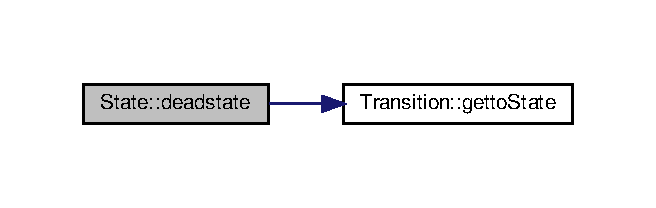
\includegraphics[width=315pt]{class_state_ab13a676e36927c127c62dba45ad7b635_cgraph}
\end{center}
\end{figure}
\mbox{\Hypertarget{class_state_ac045d201c81b6ea1ff3da734c6e286a7}\label{class_state_ac045d201c81b6ea1ff3da734c6e286a7}} 
\index{State@{State}!getn@{getn}}
\index{getn@{getn}!State@{State}}
\subsubsection{\texorpdfstring{getn()}{getn()}}
{\footnotesize\ttfamily const unsigned int \& State\+::getn (\begin{DoxyParamCaption}{ }\end{DoxyParamCaption})}



Obtener el identificador del estado. 

\begin{DoxyReturn}{Returns}
const unsigned\& \hyperlink{class_state_ac045d201c81b6ea1ff3da734c6e286a7}{State\+::getn} 
\end{DoxyReturn}


Definition at line 33 of file State.\+cpp.

Here is the caller graph for this function\+:
\nopagebreak
\begin{figure}[H]
\begin{center}
\leavevmode
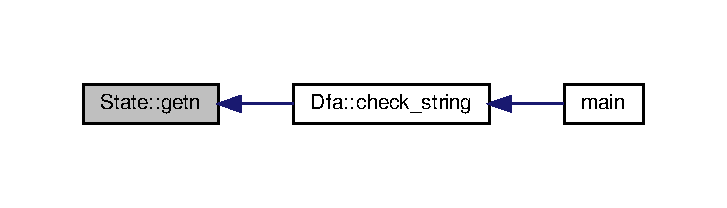
\includegraphics[width=349pt]{class_state_ac045d201c81b6ea1ff3da734c6e286a7_icgraph}
\end{center}
\end{figure}
\mbox{\Hypertarget{class_state_ac6d5a2e94f19b88ef932f84380420b35}\label{class_state_ac6d5a2e94f19b88ef932f84380420b35}} 
\index{State@{State}!getntransitions@{getntransitions}}
\index{getntransitions@{getntransitions}!State@{State}}
\subsubsection{\texorpdfstring{getntransitions()}{getntransitions()}}
{\footnotesize\ttfamily const unsigned int \& State\+::getntransitions (\begin{DoxyParamCaption}{ }\end{DoxyParamCaption})}



Obtener nº de transiciones del estado. 

\begin{DoxyReturn}{Returns}
const unsigned\& \hyperlink{class_state_ac6d5a2e94f19b88ef932f84380420b35}{State\+::getntransitions} 
\end{DoxyReturn}


Definition at line 52 of file State.\+cpp.

\mbox{\Hypertarget{class_state_aaafb1d7a01590d4b2ff055ca31028d65}\label{class_state_aaafb1d7a01590d4b2ff055ca31028d65}} 
\index{State@{State}!gettransitions@{gettransitions}}
\index{gettransitions@{gettransitions}!State@{State}}
\subsubsection{\texorpdfstring{gettransitions()}{gettransitions()}}
{\footnotesize\ttfamily const set$<$ \hyperlink{class_transition}{Transition} $>$ \& State\+::gettransitions (\begin{DoxyParamCaption}{ }\end{DoxyParamCaption})}



Obtener el conjunto de transiciones del estado. 

\begin{DoxyReturn}{Returns}
const set$<$\+Transition$>$\& 
\end{DoxyReturn}


Definition at line 61 of file State.\+cpp.

\mbox{\Hypertarget{class_state_ad701488d3ba934847dcea6222d65719e}\label{class_state_ad701488d3ba934847dcea6222d65719e}} 
\index{State@{State}!gettype@{gettype}}
\index{gettype@{gettype}!State@{State}}
\subsubsection{\texorpdfstring{gettype()}{gettype()}}
{\footnotesize\ttfamily const unsigned int \& State\+::gettype (\begin{DoxyParamCaption}{ }\end{DoxyParamCaption})}



Obtener tipo de estado, si es 1 es de aceptación. 

\begin{DoxyReturn}{Returns}
const unsigned\& \hyperlink{class_state_ad701488d3ba934847dcea6222d65719e}{State\+::gettype} 
\end{DoxyReturn}


Definition at line 43 of file State.\+cpp.

Here is the caller graph for this function\+:
\nopagebreak
\begin{figure}[H]
\begin{center}
\leavevmode
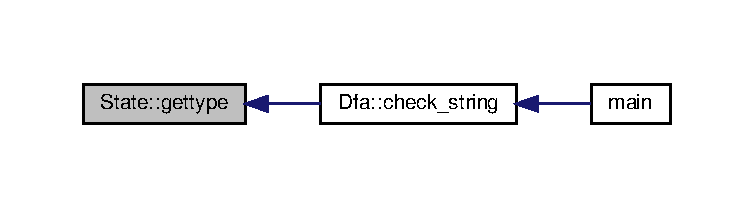
\includegraphics[width=350pt]{class_state_ad701488d3ba934847dcea6222d65719e_icgraph}
\end{center}
\end{figure}
\mbox{\Hypertarget{class_state_af93c774d8cbb27b81f2c86a0036f32d2}\label{class_state_af93c774d8cbb27b81f2c86a0036f32d2}} 
\index{State@{State}!inserttransitions@{inserttransitions}}
\index{inserttransitions@{inserttransitions}!State@{State}}
\subsubsection{\texorpdfstring{inserttransitions()}{inserttransitions()}}
{\footnotesize\ttfamily void State\+::inserttransitions (\begin{DoxyParamCaption}\item[{\hyperlink{class_transition}{Transition} \&}]{t }\end{DoxyParamCaption})}



Insertar transición. 


\begin{DoxyParams}{Parameters}
{\em t} & transición \\
\hline
\end{DoxyParams}


Definition at line 97 of file State.\+cpp.

Here is the caller graph for this function\+:
\nopagebreak
\begin{figure}[H]
\begin{center}
\leavevmode
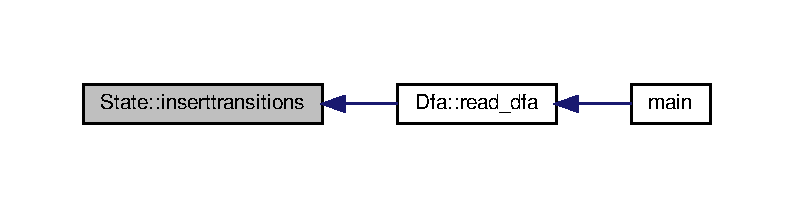
\includegraphics[width=350pt]{class_state_af93c774d8cbb27b81f2c86a0036f32d2_icgraph}
\end{center}
\end{figure}
\mbox{\Hypertarget{class_state_a7771d67d4ef98c2fd8ab7924e757781c}\label{class_state_a7771d67d4ef98c2fd8ab7924e757781c}} 
\index{State@{State}!operator$<$@{operator$<$}}
\index{operator$<$@{operator$<$}!State@{State}}
\subsubsection{\texorpdfstring{operator$<$()}{operator<()}}
{\footnotesize\ttfamily int State\+::operator$<$ (\begin{DoxyParamCaption}\item[{const \hyperlink{class_state}{State} \&}]{state }\end{DoxyParamCaption}) const}



Sobrecargar del operador $<$. 


\begin{DoxyParams}{Parameters}
{\em state} & \\
\hline
\end{DoxyParams}
\begin{DoxyReturn}{Returns}
int 
\end{DoxyReturn}


Definition at line 153 of file State.\+cpp.

\mbox{\Hypertarget{class_state_a520af8c9479e6832b07612907b2c8108}\label{class_state_a520af8c9479e6832b07612907b2c8108}} 
\index{State@{State}!operator=@{operator=}}
\index{operator=@{operator=}!State@{State}}
\subsubsection{\texorpdfstring{operator=()}{operator=()}}
{\footnotesize\ttfamily \hyperlink{class_state}{State} \& State\+::operator= (\begin{DoxyParamCaption}\item[{const \hyperlink{class_state}{State} \&}]{state }\end{DoxyParamCaption})}



Definition at line 127 of file State.\+cpp.

\mbox{\Hypertarget{class_state_a6a848174b67647a6a7a3ce467260eb7f}\label{class_state_a6a848174b67647a6a7a3ce467260eb7f}} 
\index{State@{State}!operator==@{operator==}}
\index{operator==@{operator==}!State@{State}}
\subsubsection{\texorpdfstring{operator==()}{operator==()}}
{\footnotesize\ttfamily int State\+::operator== (\begin{DoxyParamCaption}\item[{const \hyperlink{class_state}{State} \&}]{state }\end{DoxyParamCaption}) const}



Sobrecarga del operador ==. 


\begin{DoxyParams}{Parameters}
{\em state} & \\
\hline
\end{DoxyParams}
\begin{DoxyReturn}{Returns}
int 
\end{DoxyReturn}


Definition at line 140 of file State.\+cpp.

\mbox{\Hypertarget{class_state_af336de67e76fd18020cd363f82a2172e}\label{class_state_af336de67e76fd18020cd363f82a2172e}} 
\index{State@{State}!setn@{setn}}
\index{setn@{setn}!State@{State}}
\subsubsection{\texorpdfstring{setn()}{setn()}}
{\footnotesize\ttfamily void State\+::setn (\begin{DoxyParamCaption}\item[{unsigned int \&}]{n }\end{DoxyParamCaption})}



Establecer identificador del estado. 


\begin{DoxyParams}{Parameters}
{\em int} & \\
\hline
\end{DoxyParams}


Definition at line 70 of file State.\+cpp.

Here is the caller graph for this function\+:
\nopagebreak
\begin{figure}[H]
\begin{center}
\leavevmode
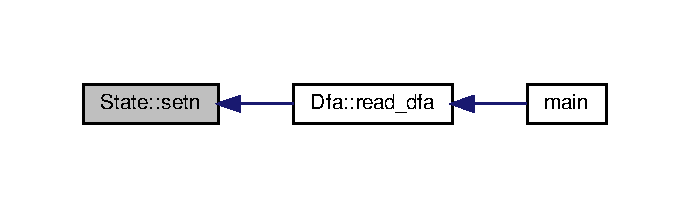
\includegraphics[width=331pt]{class_state_af336de67e76fd18020cd363f82a2172e_icgraph}
\end{center}
\end{figure}
\mbox{\Hypertarget{class_state_aae392034fc0fdf25307007548f5076d6}\label{class_state_aae392034fc0fdf25307007548f5076d6}} 
\index{State@{State}!setntransitions@{setntransitions}}
\index{setntransitions@{setntransitions}!State@{State}}
\subsubsection{\texorpdfstring{setntransitions()}{setntransitions()}}
{\footnotesize\ttfamily void State\+::setntransitions (\begin{DoxyParamCaption}\item[{unsigned int \&}]{ntransitions }\end{DoxyParamCaption})}



Establecer nº de transiciones. 


\begin{DoxyParams}{Parameters}
{\em int} & nº de transiciones \\
\hline
\end{DoxyParams}


Definition at line 88 of file State.\+cpp.

Here is the caller graph for this function\+:
\nopagebreak
\begin{figure}[H]
\begin{center}
\leavevmode
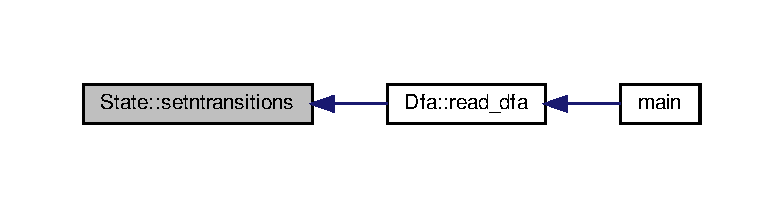
\includegraphics[width=350pt]{class_state_aae392034fc0fdf25307007548f5076d6_icgraph}
\end{center}
\end{figure}
\mbox{\Hypertarget{class_state_af24ca7913f14e5e73bcead784b4f322d}\label{class_state_af24ca7913f14e5e73bcead784b4f322d}} 
\index{State@{State}!settype@{settype}}
\index{settype@{settype}!State@{State}}
\subsubsection{\texorpdfstring{settype()}{settype()}}
{\footnotesize\ttfamily void State\+::settype (\begin{DoxyParamCaption}\item[{unsigned int \&}]{type }\end{DoxyParamCaption})}



Establecer tipo de estado. 


\begin{DoxyParams}{Parameters}
{\em int} & 1 aceptación, 0 no aceptación \\
\hline
\end{DoxyParams}


Definition at line 79 of file State.\+cpp.

Here is the caller graph for this function\+:
\nopagebreak
\begin{figure}[H]
\begin{center}
\leavevmode
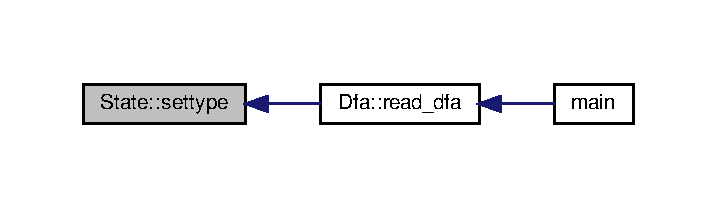
\includegraphics[width=344pt]{class_state_af24ca7913f14e5e73bcead784b4f322d_icgraph}
\end{center}
\end{figure}


\subsection{Friends And Related Function Documentation}
\mbox{\Hypertarget{class_state_a9e1d00045023572e9e6dc0d0a199e49a}\label{class_state_a9e1d00045023572e9e6dc0d0a199e49a}} 
\index{State@{State}!operator$<$$<$@{operator$<$$<$}}
\index{operator$<$$<$@{operator$<$$<$}!State@{State}}
\subsubsection{\texorpdfstring{operator$<$$<$}{operator<<}}
{\footnotesize\ttfamily ostream\& operator$<$$<$ (\begin{DoxyParamCaption}\item[{ostream \&}]{os,  }\item[{const \hyperlink{class_state}{State} \&}]{state }\end{DoxyParamCaption})\hspace{0.3cm}{\ttfamily [friend]}}



Sobrecarga del operador de salida. 


\begin{DoxyParams}{Parameters}
{\em os} & cadena resultante \\
\hline
{\em state} & \\
\hline
\end{DoxyParams}
\begin{DoxyReturn}{Returns}
ostream\& 
\end{DoxyReturn}


Definition at line 167 of file State.\+cpp.



The documentation for this class was generated from the following files\+:\begin{DoxyCompactItemize}
\item 
include/\hyperlink{_state_8hpp}{State.\+hpp}\item 
src/\hyperlink{_state_8cpp}{State.\+cpp}\end{DoxyCompactItemize}

\hypertarget{class_transition}{}\section{Transition Class Reference}
\label{class_transition}\index{Transition@{Transition}}


{\ttfamily \#include $<$Transition.\+hpp$>$}

\subsection*{Public Member Functions}
\begin{DoxyCompactItemize}
\item 
\hyperlink{class_transition_a73b44b2338b11807f77b620a3e810f92}{Transition} ()
\begin{DoxyCompactList}\small\item\em Construct a new \hyperlink{class_transition}{Transition}\+:\+: \hyperlink{class_transition}{Transition} object Constructor por defecto. \end{DoxyCompactList}\item 
\hyperlink{class_transition_ab49cf908eba3466ddcd65b144d3c2fc4}{Transition} (char, unsigned int)
\begin{DoxyCompactList}\small\item\em Construct a new \hyperlink{class_transition}{Transition}\+:\+: \hyperlink{class_transition}{Transition} object. \end{DoxyCompactList}\item 
\hyperlink{class_transition_a3a95a02ec9471b3af89c3f1b947048fc}{Transition} (const \hyperlink{class_transition}{Transition} \&t)
\begin{DoxyCompactList}\small\item\em Construct a new \hyperlink{class_transition}{Transition}\+:\+: \hyperlink{class_transition}{Transition} object Constructor de copia. \end{DoxyCompactList}\item 
const char \& \hyperlink{class_transition_a369a807fa22249a5eea8ace9d8fc10ce}{getsymbol} ()
\begin{DoxyCompactList}\small\item\em Obtener símbolo de la transición. \end{DoxyCompactList}\item 
const unsigned int \& \hyperlink{class_transition_a39709e1a9cb0b79dea569a4e1a7440c0}{getto\+State} ()
\begin{DoxyCompactList}\small\item\em Obtener estado al que va la transición. \end{DoxyCompactList}\item 
void \hyperlink{class_transition_a5a20b15b7f4ab032742ad6391190cc6e}{setsymbol} (char \&)
\begin{DoxyCompactList}\small\item\em Establecer símbolo de la transición. \end{DoxyCompactList}\item 
void \hyperlink{class_transition_ab6247c399e434db72235b6764ff80d4e}{setto\+State} (int \&)
\begin{DoxyCompactList}\small\item\em Establecer estado al que va la transición. \end{DoxyCompactList}\item 
\hyperlink{class_transition}{Transition} \& \hyperlink{class_transition_a3bb2d846d692d08eae4f1f8a43fe212d}{operator=} (const \hyperlink{class_transition}{Transition} \&t)
\begin{DoxyCompactList}\small\item\em Sobrecarga del operador =. \end{DoxyCompactList}\item 
int \hyperlink{class_transition_accb01c1a940c05f24c306c506d8988ff}{operator==} (const \hyperlink{class_transition}{Transition} \&t) const
\begin{DoxyCompactList}\small\item\em Sobrecarga del operador ==. \end{DoxyCompactList}\item 
int \hyperlink{class_transition_a6dae95e1f97bf6f39a8ae10d210e0257}{operator$<$} (const \hyperlink{class_transition}{Transition} \&t) const
\begin{DoxyCompactList}\small\item\em Sobrecarga del operador $<$. \end{DoxyCompactList}\end{DoxyCompactItemize}
\subsection*{Friends}
\begin{DoxyCompactItemize}
\item 
ostream \& \hyperlink{class_transition_ab1393a65ad3451f1fb24f8fbf1f4247f}{operator$<$$<$} (ostream \&, const \hyperlink{class_transition}{Transition} \&)
\begin{DoxyCompactList}\small\item\em Sobrecarga del operador de salida. \end{DoxyCompactList}\end{DoxyCompactItemize}


\subsection{Detailed Description}


Definition at line 8 of file Transition.\+hpp.



\subsection{Constructor \& Destructor Documentation}
\mbox{\Hypertarget{class_transition_a73b44b2338b11807f77b620a3e810f92}\label{class_transition_a73b44b2338b11807f77b620a3e810f92}} 
\index{Transition@{Transition}!Transition@{Transition}}
\index{Transition@{Transition}!Transition@{Transition}}
\subsubsection{\texorpdfstring{Transition()}{Transition()}\hspace{0.1cm}{\footnotesize\ttfamily [1/3]}}
{\footnotesize\ttfamily Transition\+::\+Transition (\begin{DoxyParamCaption}{ }\end{DoxyParamCaption})}



Construct a new \hyperlink{class_transition}{Transition}\+:\+: \hyperlink{class_transition}{Transition} object Constructor por defecto. 



Definition at line 8 of file Transition.\+cpp.

\mbox{\Hypertarget{class_transition_ab49cf908eba3466ddcd65b144d3c2fc4}\label{class_transition_ab49cf908eba3466ddcd65b144d3c2fc4}} 
\index{Transition@{Transition}!Transition@{Transition}}
\index{Transition@{Transition}!Transition@{Transition}}
\subsubsection{\texorpdfstring{Transition()}{Transition()}\hspace{0.1cm}{\footnotesize\ttfamily [2/3]}}
{\footnotesize\ttfamily Transition\+::\+Transition (\begin{DoxyParamCaption}\item[{char}]{symbol,  }\item[{unsigned int}]{to\+State }\end{DoxyParamCaption})}



Construct a new \hyperlink{class_transition}{Transition}\+:\+: \hyperlink{class_transition}{Transition} object. 


\begin{DoxyParams}{Parameters}
{\em symbol} & \\
\hline
{\em to\+State} & \\
\hline
\end{DoxyParams}


Definition at line 16 of file Transition.\+cpp.

\mbox{\Hypertarget{class_transition_a3a95a02ec9471b3af89c3f1b947048fc}\label{class_transition_a3a95a02ec9471b3af89c3f1b947048fc}} 
\index{Transition@{Transition}!Transition@{Transition}}
\index{Transition@{Transition}!Transition@{Transition}}
\subsubsection{\texorpdfstring{Transition()}{Transition()}\hspace{0.1cm}{\footnotesize\ttfamily [3/3]}}
{\footnotesize\ttfamily Transition\+::\+Transition (\begin{DoxyParamCaption}\item[{const \hyperlink{class_transition}{Transition} \&}]{t }\end{DoxyParamCaption})}



Construct a new \hyperlink{class_transition}{Transition}\+:\+: \hyperlink{class_transition}{Transition} object Constructor de copia. 


\begin{DoxyParams}{Parameters}
{\em t} & \\
\hline
\end{DoxyParams}


Definition at line 27 of file Transition.\+cpp.



\subsection{Member Function Documentation}
\mbox{\Hypertarget{class_transition_a369a807fa22249a5eea8ace9d8fc10ce}\label{class_transition_a369a807fa22249a5eea8ace9d8fc10ce}} 
\index{Transition@{Transition}!getsymbol@{getsymbol}}
\index{getsymbol@{getsymbol}!Transition@{Transition}}
\subsubsection{\texorpdfstring{getsymbol()}{getsymbol()}}
{\footnotesize\ttfamily const char \& Transition\+::getsymbol (\begin{DoxyParamCaption}{ }\end{DoxyParamCaption})}



Obtener símbolo de la transición. 

\begin{DoxyReturn}{Returns}
const char\& 
\end{DoxyReturn}


Definition at line 36 of file Transition.\+cpp.

\mbox{\Hypertarget{class_transition_a39709e1a9cb0b79dea569a4e1a7440c0}\label{class_transition_a39709e1a9cb0b79dea569a4e1a7440c0}} 
\index{Transition@{Transition}!getto\+State@{getto\+State}}
\index{getto\+State@{getto\+State}!Transition@{Transition}}
\subsubsection{\texorpdfstring{getto\+State()}{gettoState()}}
{\footnotesize\ttfamily const unsigned int \& Transition\+::getto\+State (\begin{DoxyParamCaption}{ }\end{DoxyParamCaption})}



Obtener estado al que va la transición. 

\begin{DoxyReturn}{Returns}
const unsigned\& \hyperlink{class_transition_a39709e1a9cb0b79dea569a4e1a7440c0}{Transition\+::getto\+State} 
\end{DoxyReturn}


Definition at line 45 of file Transition.\+cpp.

Here is the caller graph for this function\+:
\nopagebreak
\begin{figure}[H]
\begin{center}
\leavevmode
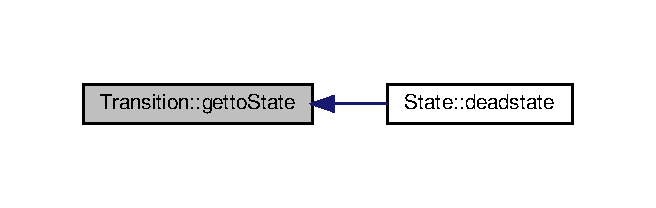
\includegraphics[width=315pt]{class_transition_a39709e1a9cb0b79dea569a4e1a7440c0_icgraph}
\end{center}
\end{figure}
\mbox{\Hypertarget{class_transition_a6dae95e1f97bf6f39a8ae10d210e0257}\label{class_transition_a6dae95e1f97bf6f39a8ae10d210e0257}} 
\index{Transition@{Transition}!operator$<$@{operator$<$}}
\index{operator$<$@{operator$<$}!Transition@{Transition}}
\subsubsection{\texorpdfstring{operator$<$()}{operator<()}}
{\footnotesize\ttfamily int Transition\+::operator$<$ (\begin{DoxyParamCaption}\item[{const \hyperlink{class_transition}{Transition} \&}]{t }\end{DoxyParamCaption}) const}



Sobrecarga del operador $<$. 


\begin{DoxyParams}{Parameters}
{\em t} & \\
\hline
\end{DoxyParams}
\begin{DoxyReturn}{Returns}
int 1 true, 0 false 
\end{DoxyReturn}


Definition at line 101 of file Transition.\+cpp.

\mbox{\Hypertarget{class_transition_a3bb2d846d692d08eae4f1f8a43fe212d}\label{class_transition_a3bb2d846d692d08eae4f1f8a43fe212d}} 
\index{Transition@{Transition}!operator=@{operator=}}
\index{operator=@{operator=}!Transition@{Transition}}
\subsubsection{\texorpdfstring{operator=()}{operator=()}}
{\footnotesize\ttfamily \hyperlink{class_transition}{Transition} \& Transition\+::operator= (\begin{DoxyParamCaption}\item[{const \hyperlink{class_transition}{Transition} \&}]{t }\end{DoxyParamCaption})}



Sobrecarga del operador =. 


\begin{DoxyParams}{Parameters}
{\em t} & \\
\hline
\end{DoxyParams}
\begin{DoxyReturn}{Returns}
\hyperlink{class_transition}{Transition}\& 
\end{DoxyReturn}


Definition at line 73 of file Transition.\+cpp.

\mbox{\Hypertarget{class_transition_accb01c1a940c05f24c306c506d8988ff}\label{class_transition_accb01c1a940c05f24c306c506d8988ff}} 
\index{Transition@{Transition}!operator==@{operator==}}
\index{operator==@{operator==}!Transition@{Transition}}
\subsubsection{\texorpdfstring{operator==()}{operator==()}}
{\footnotesize\ttfamily int Transition\+::operator== (\begin{DoxyParamCaption}\item[{const \hyperlink{class_transition}{Transition} \&}]{t }\end{DoxyParamCaption}) const}



Sobrecarga del operador ==. 


\begin{DoxyParams}{Parameters}
{\em t} & \\
\hline
\end{DoxyParams}
\begin{DoxyReturn}{Returns}
int 1 true, 0 false 
\end{DoxyReturn}


Definition at line 85 of file Transition.\+cpp.

\mbox{\Hypertarget{class_transition_a5a20b15b7f4ab032742ad6391190cc6e}\label{class_transition_a5a20b15b7f4ab032742ad6391190cc6e}} 
\index{Transition@{Transition}!setsymbol@{setsymbol}}
\index{setsymbol@{setsymbol}!Transition@{Transition}}
\subsubsection{\texorpdfstring{setsymbol()}{setsymbol()}}
{\footnotesize\ttfamily void Transition\+::setsymbol (\begin{DoxyParamCaption}\item[{char \&}]{symbol }\end{DoxyParamCaption})}



Establecer símbolo de la transición. 


\begin{DoxyParams}{Parameters}
{\em symbol} & \\
\hline
\end{DoxyParams}


Definition at line 54 of file Transition.\+cpp.

\mbox{\Hypertarget{class_transition_ab6247c399e434db72235b6764ff80d4e}\label{class_transition_ab6247c399e434db72235b6764ff80d4e}} 
\index{Transition@{Transition}!setto\+State@{setto\+State}}
\index{setto\+State@{setto\+State}!Transition@{Transition}}
\subsubsection{\texorpdfstring{setto\+State()}{settoState()}}
{\footnotesize\ttfamily void Transition\+::setto\+State (\begin{DoxyParamCaption}\item[{int \&}]{to\+State }\end{DoxyParamCaption})}



Establecer estado al que va la transición. 


\begin{DoxyParams}{Parameters}
{\em to\+State} & \\
\hline
\end{DoxyParams}


Definition at line 63 of file Transition.\+cpp.



\subsection{Friends And Related Function Documentation}
\mbox{\Hypertarget{class_transition_ab1393a65ad3451f1fb24f8fbf1f4247f}\label{class_transition_ab1393a65ad3451f1fb24f8fbf1f4247f}} 
\index{Transition@{Transition}!operator$<$$<$@{operator$<$$<$}}
\index{operator$<$$<$@{operator$<$$<$}!Transition@{Transition}}
\subsubsection{\texorpdfstring{operator$<$$<$}{operator<<}}
{\footnotesize\ttfamily ostream\& operator$<$$<$ (\begin{DoxyParamCaption}\item[{ostream \&}]{os,  }\item[{const \hyperlink{class_transition}{Transition} \&}]{transition }\end{DoxyParamCaption})\hspace{0.3cm}{\ttfamily [friend]}}



Sobrecarga del operador de salida. 


\begin{DoxyParams}{Parameters}
{\em os} & Cadena resultante \\
\hline
{\em transition} & \\
\hline
\end{DoxyParams}
\begin{DoxyReturn}{Returns}
ostream\& 
\end{DoxyReturn}


Definition at line 118 of file Transition.\+cpp.



The documentation for this class was generated from the following files\+:\begin{DoxyCompactItemize}
\item 
include/\hyperlink{_transition_8hpp}{Transition.\+hpp}\item 
src/\hyperlink{_transition_8cpp}{Transition.\+cpp}\end{DoxyCompactItemize}

\chapter{File Documentation}
\hypertarget{_dfa_8hpp}{}\section{include/\+Dfa.hpp File Reference}
\label{_dfa_8hpp}\index{include/\+Dfa.\+hpp@{include/\+Dfa.\+hpp}}
{\ttfamily \#include $<$sstream$>$}\newline
{\ttfamily \#include $<$fstream$>$}\newline
{\ttfamily \#include $<$string$>$}\newline
{\ttfamily \#include \char`\"{}State.\+hpp\char`\"{}}\newline
Include dependency graph for Dfa.\+hpp\+:
\nopagebreak
\begin{figure}[H]
\begin{center}
\leavevmode
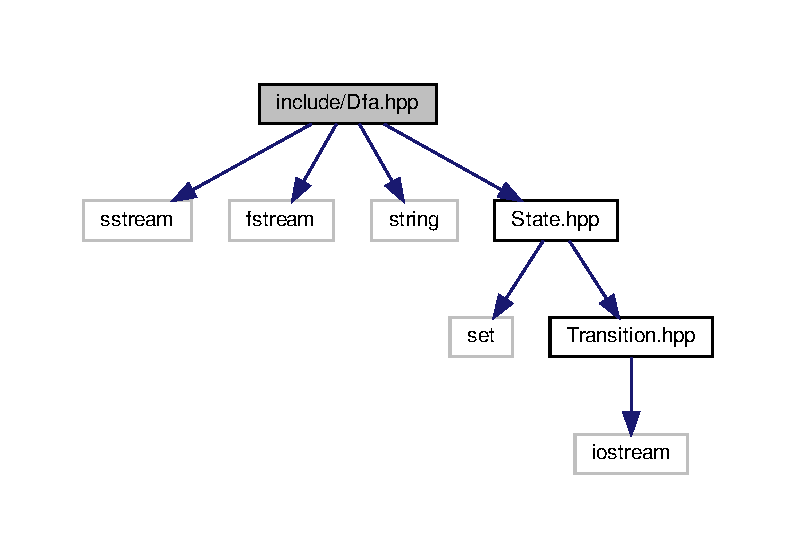
\includegraphics[width=350pt]{_dfa_8hpp__incl}
\end{center}
\end{figure}
This graph shows which files directly or indirectly include this file\+:
\nopagebreak
\begin{figure}[H]
\begin{center}
\leavevmode
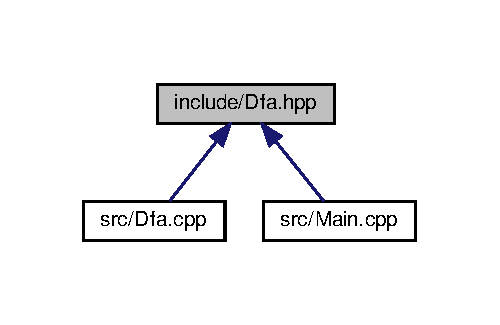
\includegraphics[width=240pt]{_dfa_8hpp__dep__incl}
\end{center}
\end{figure}
\subsection*{Classes}
\begin{DoxyCompactItemize}
\item 
class \hyperlink{class_dfa}{Dfa}
\end{DoxyCompactItemize}

\hypertarget{_state_8hpp}{}\section{include/\+State.hpp File Reference}
\label{_state_8hpp}\index{include/\+State.\+hpp@{include/\+State.\+hpp}}
{\ttfamily \#include $<$set$>$}\newline
{\ttfamily \#include \char`\"{}Transition.\+hpp\char`\"{}}\newline
Include dependency graph for State.\+hpp\+:
\nopagebreak
\begin{figure}[H]
\begin{center}
\leavevmode
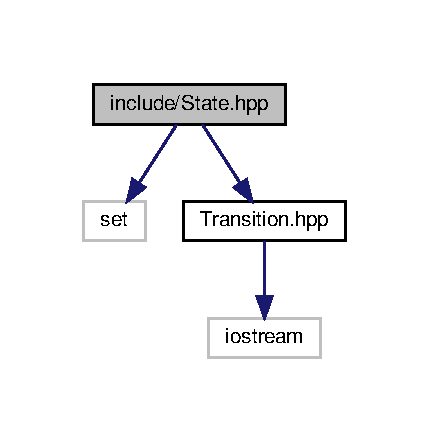
\includegraphics[width=206pt]{_state_8hpp__incl}
\end{center}
\end{figure}
This graph shows which files directly or indirectly include this file\+:
\nopagebreak
\begin{figure}[H]
\begin{center}
\leavevmode
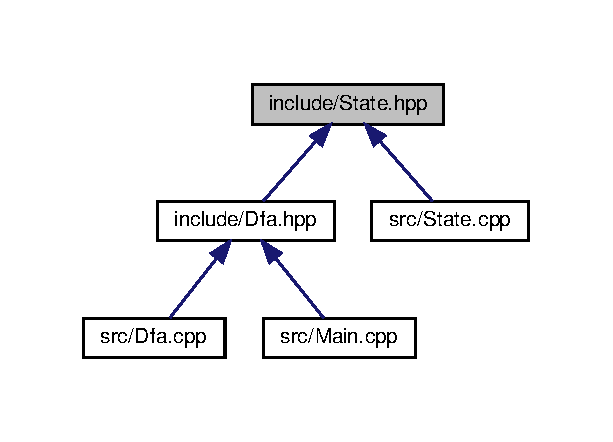
\includegraphics[width=294pt]{_state_8hpp__dep__incl}
\end{center}
\end{figure}
\subsection*{Classes}
\begin{DoxyCompactItemize}
\item 
class \hyperlink{class_state}{State}
\end{DoxyCompactItemize}

\hypertarget{_transition_8hpp}{}\section{include/\+Transition.hpp File Reference}
\label{_transition_8hpp}\index{include/\+Transition.\+hpp@{include/\+Transition.\+hpp}}
{\ttfamily \#include $<$iostream$>$}\newline
Include dependency graph for Transition.\+hpp\+:
\nopagebreak
\begin{figure}[H]
\begin{center}
\leavevmode
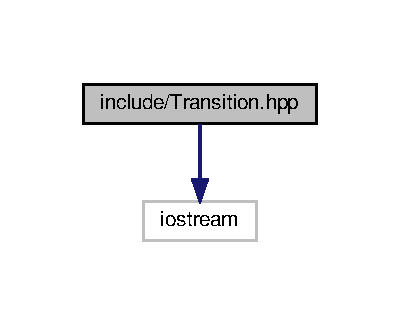
\includegraphics[width=192pt]{_transition_8hpp__incl}
\end{center}
\end{figure}
This graph shows which files directly or indirectly include this file\+:
\nopagebreak
\begin{figure}[H]
\begin{center}
\leavevmode
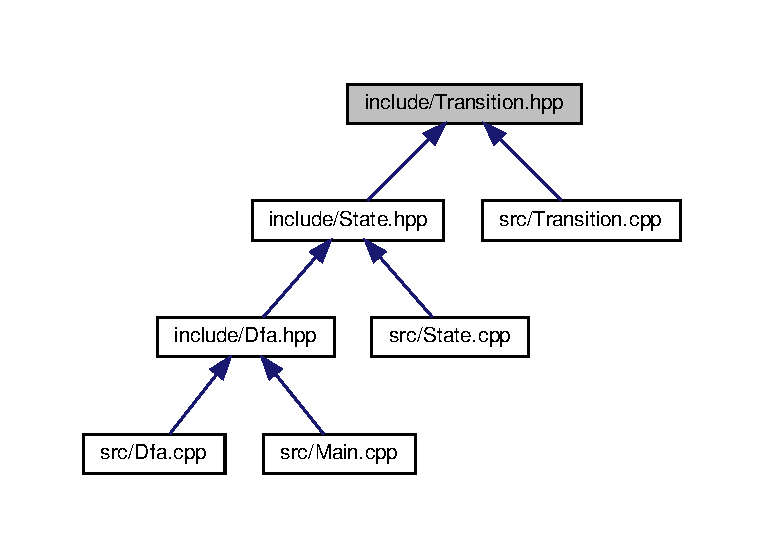
\includegraphics[width=350pt]{_transition_8hpp__dep__incl}
\end{center}
\end{figure}
\subsection*{Classes}
\begin{DoxyCompactItemize}
\item 
class \hyperlink{class_transition}{Transition}
\end{DoxyCompactItemize}

\hypertarget{_r_e_a_d_m_e_8md}{}\section{R\+E\+A\+D\+M\+E.\+md File Reference}
\label{_r_e_a_d_m_e_8md}\index{R\+E\+A\+D\+M\+E.\+md@{R\+E\+A\+D\+M\+E.\+md}}

\hypertarget{_dfa_8cpp}{}\section{src/\+Dfa.cpp File Reference}
\label{_dfa_8cpp}\index{src/\+Dfa.\+cpp@{src/\+Dfa.\+cpp}}
{\ttfamily \#include \char`\"{}../include/\+Dfa.\+hpp\char`\"{}}\newline
Include dependency graph for Dfa.\+cpp\+:
\nopagebreak
\begin{figure}[H]
\begin{center}
\leavevmode
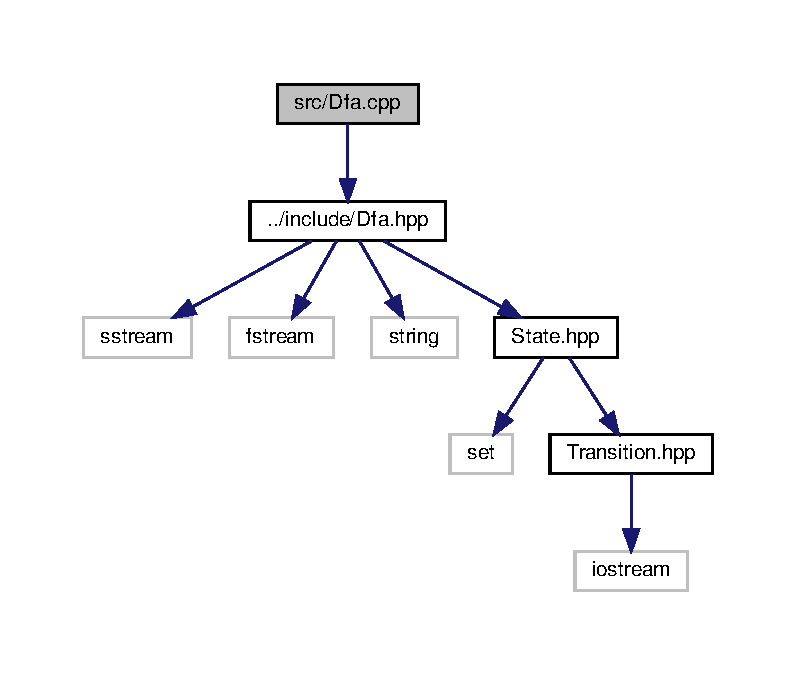
\includegraphics[width=350pt]{_dfa_8cpp__incl}
\end{center}
\end{figure}
\subsection*{Functions}
\begin{DoxyCompactItemize}
\item 
ostream \& \hyperlink{_dfa_8cpp_ae4bcdc6c0f5c2374f14902fd5e073c7d}{operator$<$$<$} (ostream \&os, const \hyperlink{class_dfa}{Dfa} \&dfa)
\end{DoxyCompactItemize}


\subsection{Function Documentation}
\mbox{\Hypertarget{_dfa_8cpp_ae4bcdc6c0f5c2374f14902fd5e073c7d}\label{_dfa_8cpp_ae4bcdc6c0f5c2374f14902fd5e073c7d}} 
\index{Dfa.\+cpp@{Dfa.\+cpp}!operator$<$$<$@{operator$<$$<$}}
\index{operator$<$$<$@{operator$<$$<$}!Dfa.\+cpp@{Dfa.\+cpp}}
\subsubsection{\texorpdfstring{operator$<$$<$()}{operator<<()}}
{\footnotesize\ttfamily ostream\& operator$<$$<$ (\begin{DoxyParamCaption}\item[{ostream \&}]{os,  }\item[{const \hyperlink{class_dfa}{Dfa} \&}]{dfa }\end{DoxyParamCaption})}



Definition at line 234 of file Dfa.\+cpp.


\hypertarget{_main_8cpp}{}\section{src/\+Main.cpp File Reference}
\label{_main_8cpp}\index{src/\+Main.\+cpp@{src/\+Main.\+cpp}}
{\ttfamily \#include \char`\"{}../include/\+Dfa.\+hpp\char`\"{}}\newline
{\ttfamily \#include $<$cstdlib$>$}\newline
{\ttfamily \#include $<$istream$>$}\newline
Include dependency graph for Main.\+cpp\+:
\nopagebreak
\begin{figure}[H]
\begin{center}
\leavevmode
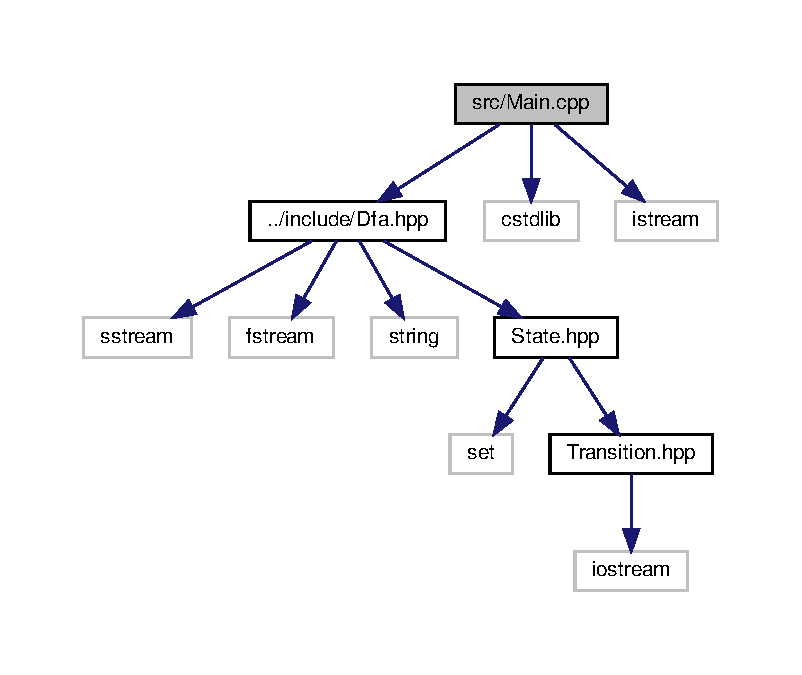
\includegraphics[width=350pt]{_main_8cpp__incl}
\end{center}
\end{figure}
\subsection*{Functions}
\begin{DoxyCompactItemize}
\item 
int \hyperlink{_main_8cpp_ae66f6b31b5ad750f1fe042a706a4e3d4}{main} ()
\end{DoxyCompactItemize}


\subsection{Function Documentation}
\mbox{\Hypertarget{_main_8cpp_ae66f6b31b5ad750f1fe042a706a4e3d4}\label{_main_8cpp_ae66f6b31b5ad750f1fe042a706a4e3d4}} 
\index{Main.\+cpp@{Main.\+cpp}!main@{main}}
\index{main@{main}!Main.\+cpp@{Main.\+cpp}}
\subsubsection{\texorpdfstring{main()}{main()}}
{\footnotesize\ttfamily int main (\begin{DoxyParamCaption}{ }\end{DoxyParamCaption})}



Definition at line 14 of file Main.\+cpp.

Here is the call graph for this function\+:
\nopagebreak
\begin{figure}[H]
\begin{center}
\leavevmode
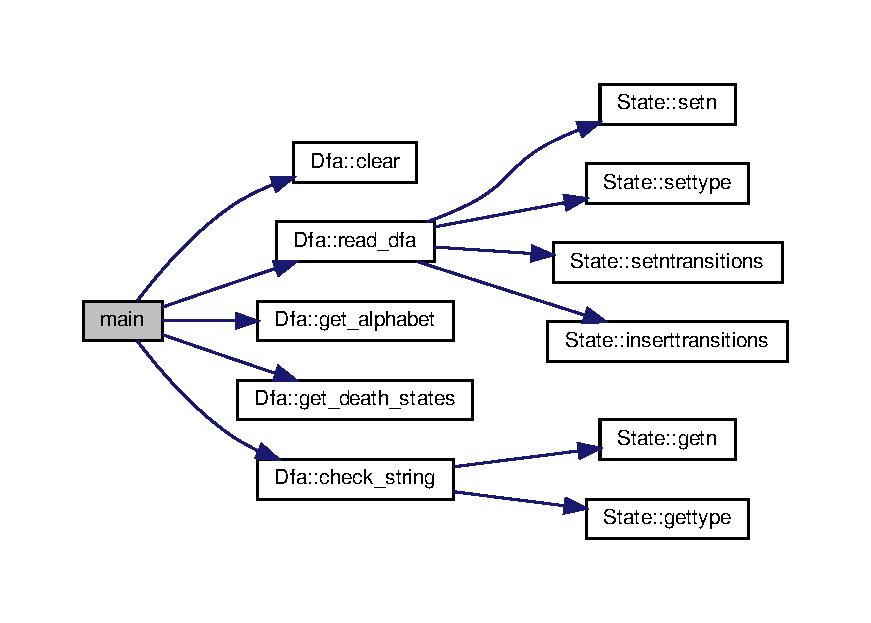
\includegraphics[width=350pt]{_main_8cpp_ae66f6b31b5ad750f1fe042a706a4e3d4_cgraph}
\end{center}
\end{figure}

\hypertarget{_state_8cpp}{}\section{src/\+State.cpp File Reference}
\label{_state_8cpp}\index{src/\+State.\+cpp@{src/\+State.\+cpp}}
{\ttfamily \#include \char`\"{}../include/\+State.\+hpp\char`\"{}}\newline
Include dependency graph for State.\+cpp\+:
\nopagebreak
\begin{figure}[H]
\begin{center}
\leavevmode
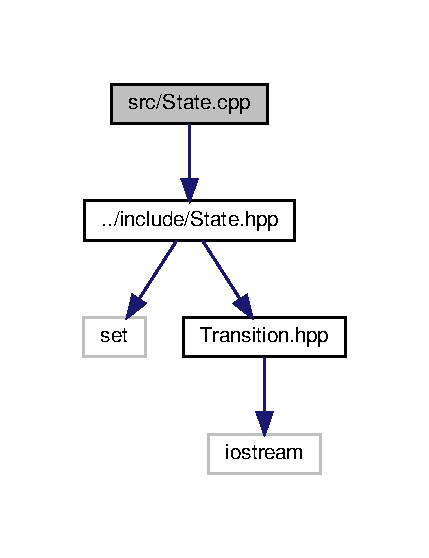
\includegraphics[width=206pt]{_state_8cpp__incl}
\end{center}
\end{figure}
\subsection*{Functions}
\begin{DoxyCompactItemize}
\item 
ostream \& \hyperlink{_state_8cpp_a28462fe8a40ddca879c3bb4abbea5e13}{operator$<$$<$} (ostream \&os, const \hyperlink{class_state}{State} \&state)
\begin{DoxyCompactList}\small\item\em Sobrecarga del operador de salida. \end{DoxyCompactList}\end{DoxyCompactItemize}


\subsection{Function Documentation}
\mbox{\Hypertarget{_state_8cpp_a28462fe8a40ddca879c3bb4abbea5e13}\label{_state_8cpp_a28462fe8a40ddca879c3bb4abbea5e13}} 
\index{State.\+cpp@{State.\+cpp}!operator$<$$<$@{operator$<$$<$}}
\index{operator$<$$<$@{operator$<$$<$}!State.\+cpp@{State.\+cpp}}
\subsubsection{\texorpdfstring{operator$<$$<$()}{operator<<()}}
{\footnotesize\ttfamily ostream\& operator$<$$<$ (\begin{DoxyParamCaption}\item[{ostream \&}]{os,  }\item[{const \hyperlink{class_state}{State} \&}]{state }\end{DoxyParamCaption})}



Sobrecarga del operador de salida. 


\begin{DoxyParams}{Parameters}
{\em os} & cadena resultante \\
\hline
{\em state} & \\
\hline
\end{DoxyParams}
\begin{DoxyReturn}{Returns}
ostream\& 
\end{DoxyReturn}


Definition at line 167 of file State.\+cpp.


\hypertarget{_transition_8cpp}{}\section{src/\+Transition.cpp File Reference}
\label{_transition_8cpp}\index{src/\+Transition.\+cpp@{src/\+Transition.\+cpp}}
{\ttfamily \#include \char`\"{}../include/\+Transition.\+hpp\char`\"{}}\newline
Include dependency graph for Transition.\+cpp\+:
\nopagebreak
\begin{figure}[H]
\begin{center}
\leavevmode
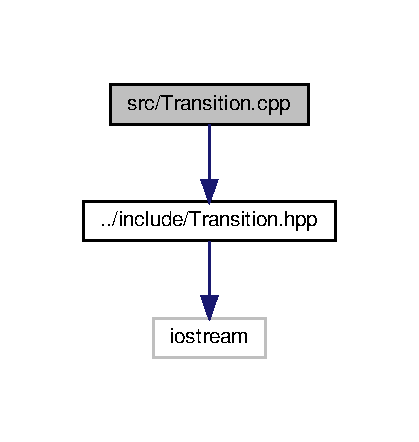
\includegraphics[width=201pt]{_transition_8cpp__incl}
\end{center}
\end{figure}
\subsection*{Functions}
\begin{DoxyCompactItemize}
\item 
ostream \& \hyperlink{_transition_8cpp_abdbf837e09379a17a12b260699e15b4d}{operator$<$$<$} (ostream \&os, const \hyperlink{class_transition}{Transition} \&transition)
\begin{DoxyCompactList}\small\item\em Sobrecarga del operador de salida. \end{DoxyCompactList}\end{DoxyCompactItemize}


\subsection{Function Documentation}
\mbox{\Hypertarget{_transition_8cpp_abdbf837e09379a17a12b260699e15b4d}\label{_transition_8cpp_abdbf837e09379a17a12b260699e15b4d}} 
\index{Transition.\+cpp@{Transition.\+cpp}!operator$<$$<$@{operator$<$$<$}}
\index{operator$<$$<$@{operator$<$$<$}!Transition.\+cpp@{Transition.\+cpp}}
\subsubsection{\texorpdfstring{operator$<$$<$()}{operator<<()}}
{\footnotesize\ttfamily ostream\& operator$<$$<$ (\begin{DoxyParamCaption}\item[{ostream \&}]{os,  }\item[{const \hyperlink{class_transition}{Transition} \&}]{transition }\end{DoxyParamCaption})}



Sobrecarga del operador de salida. 


\begin{DoxyParams}{Parameters}
{\em os} & Cadena resultante \\
\hline
{\em transition} & \\
\hline
\end{DoxyParams}
\begin{DoxyReturn}{Returns}
ostream\& 
\end{DoxyReturn}


Definition at line 118 of file Transition.\+cpp.


%--- End generated contents ---

% Index
\backmatter
\newpage
\phantomsection
\clearemptydoublepage
\addcontentsline{toc}{chapter}{Index}
\printindex

\end{document}
